% Author:Zhuming Shi, Peking University
% Theme from https://github.com/matze/mtheme

\documentclass[12pt,AutoFakeBold,aspectratio=43,mathserif]{beamer}
\usepackage[english]{babel}

\usetheme{metropolis}
\metroset{block=fill}
\usepackage{fontspec}% 控制字体
\setmainfont{Times New Roman}% 英文字体
\newfontfamily\arial{Arial}% Arial字体

\usepackage{xeCJK} % 中文支持
\setCJKmainfont{SimSun} % 中文字体
\setCJKsansfont{SimHei}
\XeTeXlinebreaklocale "zh"%中文自动换行
\XeTeXlinebreakskip = 0pt plus 1pt%中文自动换行

\usepackage{graphicx}
\usepackage{subfigure}
\usepackage{caption}

\usepackage{amsthm,amsmath,amssymb,mathrsfs}% 数学符号和花体支持
\usepackage{booktabs}% 绘制三线表
\usepackage{latexsym}% 绘制特殊数学符号
\usepackage{siunitx}% 数学模式中使用SI单位

\usepackage[version=3]{mhchem}% 化学反应式
\usepackage{epstopdf}% 插入ChemDraw的.eps结构图

% 代码环境
\usepackage{listings}
\usepackage{color}

\useoutertheme{infolines}

\definecolor{dkgreen}{rgb}{0,0.6,0}
\definecolor{gray}{rgb}{0.5,0.5,0.5}
\definecolor{mauve}{rgb}{0.58,0,0.82}

\lstset{frame=tb,
  language=c++,
  aboveskip=3mm,
  belowskip=3mm,
  showstringspaces=false,
  columns=flexible,
  basicstyle={\small\ttfamily},
  numbers=none,
  numberstyle=\tiny\color{gray},
  keywordstyle=\color{blue},
  commentstyle=\color{dkgreen},
  stringstyle=\color{mauve},
  breaklines=true,
  breakatwhitespace=true,
  tabsize=3
}

\setbeamerfont{footnote}{size=\tiny}

\newcommand{\unknow}[1]{{\arial \textbf{#1}}}%未知化合物格式
\newcommand{\substance}[1]{\textbf{\emph{#1}}}%矿物名称格式

% \setbeamertemplate{background}{\includegraphics[height=\paperheight]{figures/misaka1080.png}}

\makeatletter 
\renewcommand{\@thesubfigure}{\hskip\subfiglabelskip}
\makeatother

\title{从控制论到计算机}
\author{前沿第四组}
\date{10月22日}

\begin{document}
    \begin{frame}
        % \frametitle{}
        \titlepage
    
    \end{frame}
    \frame{\frametitle{Outline}\tableofcontents[hideallsubsections]}
    
    \section{机构与变异度}

    \section{调节与控制}

    \begin{frame}{浅谈调节}
        \begin{itemize}
                \item 调节作用堵塞了干扰源传向基本变量的变异度
                \item 例:恒温淋浴设备
               \begin{figure}[H]
                \centering
                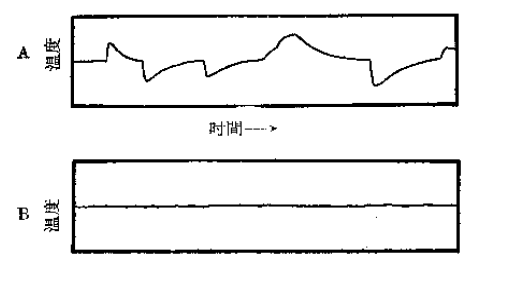
\includegraphics[width=.6\textwidth]{figures/pic1.png}
                \end{figure}
        \end{itemize}
        
    \end{frame}
    \begin{frame}{必须变异度}
        \begin{itemize}
              \item D和R进行游戏, R在D之后做动作
              \begin{figure}[H]
                \centering
                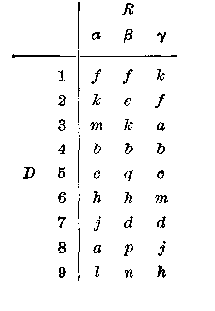
\includegraphics[width=.4\textwidth]{figures/pic2.png}
                \end{figure}
                \item 结局的变异度不能小于$\frac{D\text{的变异度}}{R\text{的变异度}}=\frac{9}{3}$
                \item 只有变异度才能消灭变异度!
        \end{itemize}
    \end{frame}
    \begin{frame}{必须变异度率}
        \begin{itemize}
                \item 若调节器R已给定, 则结局E的熵不小于干扰D的熵
                \item $H_R(E)\geq H_R(D)$
                \item 其他附加条件(如噪声、复合干扰、调节的误差等)都可以视作R的一部分
        \end{itemize}
    \end{frame}
    \begin{frame}{马尔可夫型机器}
        \begin{itemize}
                \item 非确定性机器: 更加曲折但更加鲁棒地趋向平衡状态
                \begin{figure}[H]
                \centering
                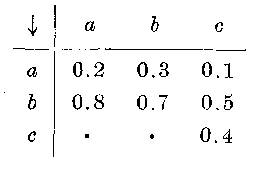
\includegraphics[width=.6\textwidth]{figures/pic3.png}
                \end{figure}
                \item 例: 捕蝇纸对于房间中苍蝇的作用
        \end{itemize}
        
    \end{frame}
      
    \begin{frame}{其他调节}
        \begin{itemize}
                \item 特大系统: 系统T相对于调节器R来说很大, 怎么办 ?
                \item[1] 约束
                \begin{figure}[H]
                \centering
                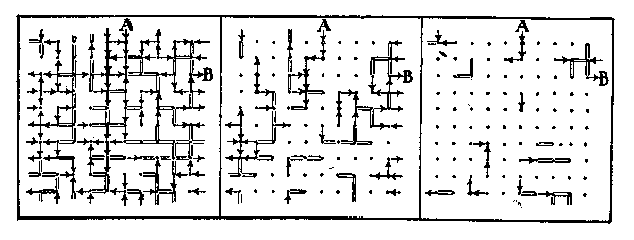
\includegraphics[width=.6\textwidth]{figures/pic4.png}
                \end{figure}
                \item[2] 关注重复干扰的总结果
                \item[3] 功率放大器
        \end{itemize}
    \end{frame}

    \section{从控制论到计算机}
    \subsection{控制科学(学科)\& 计算机}
    \begin{frame}
        \frametitle{控制科学(学科)\& 计算机}
        \pause
        控制科学和计算机是两门学科. \\
        在隔壁,研究控制科学的学科是「自动化」。
        \begin{figure}[htbp]
            \caption{清华大学自动化专业本科课程}
            \setlength{\abovecaptionskip}{0.cm}
            \setlength{\belowcaptionskip}{-0.cm}
            \centering
            \vspace{-0.3cm}
            \setlength{\abovecaptionskip}{0.cm}
            \setlength{\belowcaptionskip}{-0.cm}
            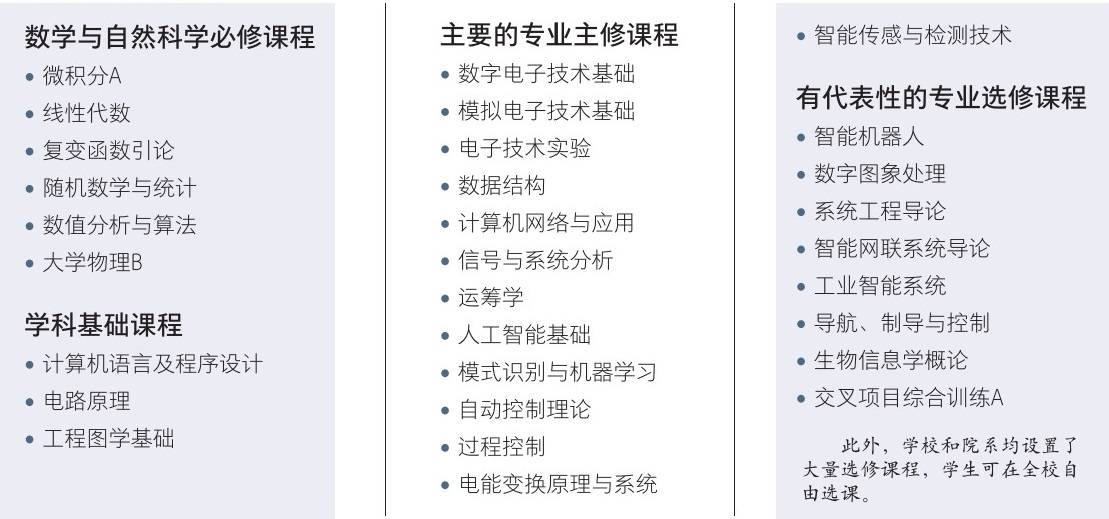
\includegraphics[width=0.9\textwidth]{figures/3-1.jpg}
        \end{figure}
    \end{frame}
    \subsection{控制论 \& 控制理论}
    \begin{frame}
        \frametitle{控制论 \& 控制理论}
        \begin{block}{\textnormal{「控制论」与「控制理论」是一回事吗?}}
        \end{block} \pause
        \footnotesize
        控制论(Cybernetics)与控制理论(Control Theory)是两个不同的概念。 \\
        有的人简单地、片面地认为,控制论是软科学,像哲学;控制理论是硬科学,像数学。这是造成控制论和控制理论概念混乱和理解变形的主要原因。 \\
        \begin{itemize}
            \item 控制理论涉及工程过程和机器中动力系统的控制。目的是开发一种控制模型,以最优方式使用控制动作来控制此类系统,而不会出现延迟或超调,并确保控制稳定性。\pause
            \item 控制论是一种探索调节系统——其结构、约束和可能性的跨学科方法。\pause
        \end{itemize}
        控制论将控制系统作为一个在整体概念进行研究,而控制理论着重于信息因素,研究系统中各部分的相互作用以及系统的结构。
        \pause
        
    
    \end{frame}
    \subsection{控制论 \& 计算机}
    \begin{frame}
        \frametitle{控制论和计算机的关系}
        \begin{block}{\textnormal{为什么控制论和计算机有关系?}} \end{block} \pause
        \begin{columns}
            \begin{column}{.5\linewidth}
                \begin{itemize}
                    \item  \footnotesize 控制论研究的首要的一个理论,就是要建立起一个有效的理论,能模拟人和其他生物行为的各个方面,并且依靠这种理论能制造出人工智能,计算机的出现提供了一个新的思路。 \pause
                    \item  \footnotesize 控制论是一个综合的学科,它想要提出一种通用的方法解释所有其他学科。实际中控制论研究的对象更多是社会学科,而计算机可以将这些学科联系起来。 
                \end{itemize}
            \end{column}
            \begin{column}{.5\linewidth}
                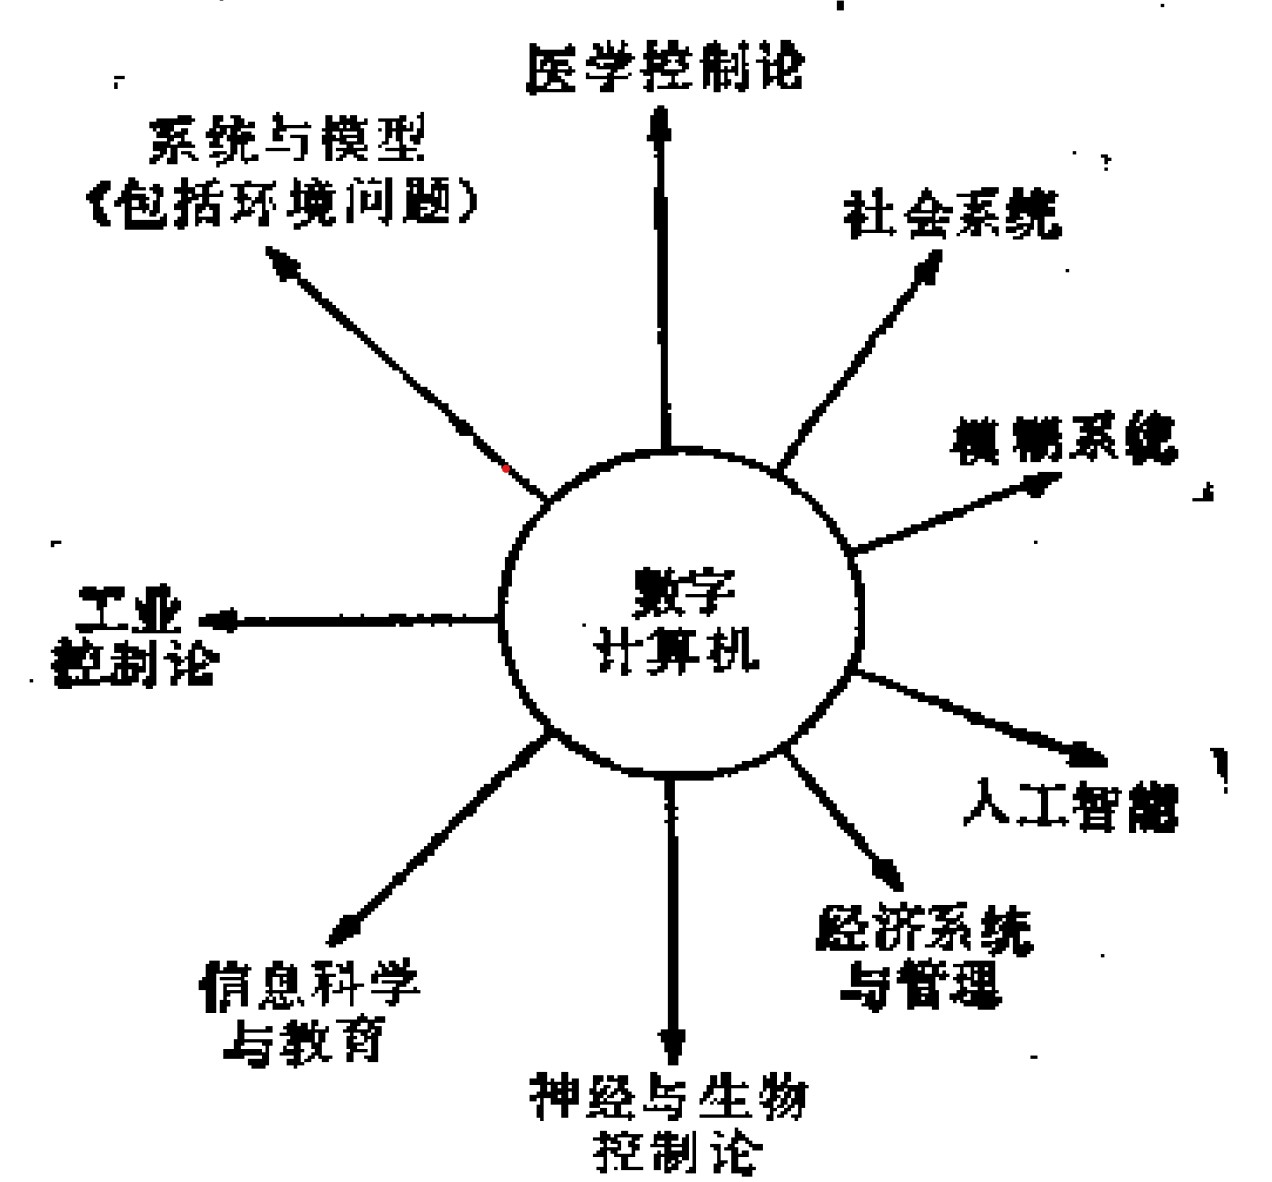
\includegraphics[width=.4\paperwidth]{figures/3-3.jpg}
            \end{column}
        \end{columns}
        
    \end{frame}
    \begin{frame}
        \frametitle{控制论和计算机的关系}
        控制论对计算机的发展也有促进的作用(实际上是控制理论) \pause
        \begin{itemize}
            \item 在CPU内部引入流水线控制技术

            \item 并行、动态分支预测、可编程控制器
        \end{itemize}
        
    \end{frame}
    \begin{frame}
        \frametitle{控制论 \& 强化学习}
        强化学习和控制理论有着很深的联系。 \pause
        \begin{itemize}
            \item  强化学习和控制理论都是研究利用过去的信息来强化未来操纵的动态系统。\pause
            \item  强化学习和控制理论的目的都是设计一个系统,其能够使用高度结构化的感知信息,做出规划和控制以适应环境变化,同时在遇到新场景时做好保障。因此,可以使用强化学习的思想和算法来解决控制系统的问题。 
        \end{itemize}
    \end{frame}
    \begin{frame}
        \frametitle{控制论 \& 强化学习}
        \begin{columns}
            \begin{column}{.4\linewidth}
                强化学习策略的行为(即策略如何观察环境并以最佳方式生成动作来完成任务)和控制系统中控制器的操作是类似的,如图。 \\
                (上图是强化学习,下图是控制器,线的颜色相同的部分是对应的关系)
            \end{column}
            \begin{column}{.5\linewidth}
                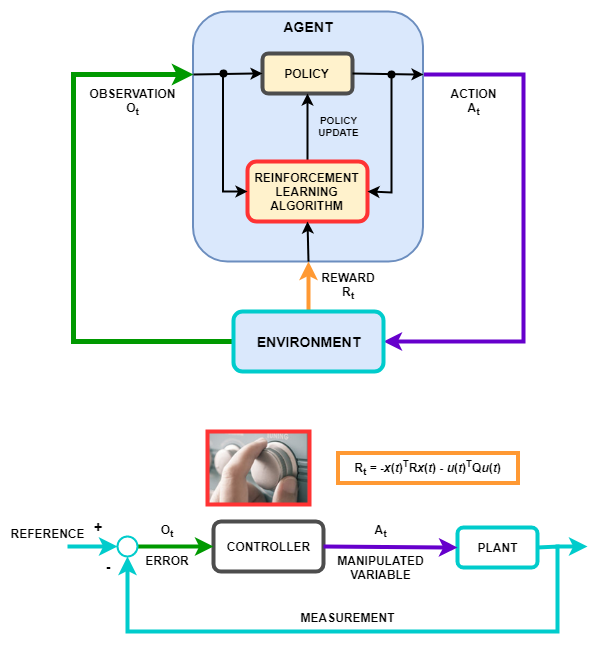
\includegraphics[width=.5\paperwidth]{figures/rl_for_control_systems.png}
            \end{column}
        \end{columns}
    \end{frame}
    \subsection{控制论应用举例}
    \begin{frame}
        \frametitle{控制论应用举例}
        接下来是控制论应用的一些例子。
    \end{frame}
    \begin{frame}
        \frametitle{网络控制}
        \footnotesize 网络控制是一个很大的领域,涉及许多主题,包括路由、数据缓存和电源管理。这些控制问题的一些特点使它们非常具有挑战性: \pause
        \begin{itemize}
            \item  系统的超大规模:Internet可能是人类所建立的最大的反馈控制系统。
            \item  控制问题的分散化本质:必须快速做出局部决策,并且仅基于局部信息。
            \item  其它:比如对服务质量的不同要求等。
        \end{itemize} \pause
        网络控制下一阶段将涉及更多的物理环境和对网络控制的增加使用,需要通信、计算和控制的融合。 \\ \pause
        另一个可能的发展方向:目前的网络控制系统几乎普遍基于同步、定时系统来避免数据丢失,我们是否可以开发一个理论和实践控制系统,在一个分布式的、异步的、基于分组的环境中运行,这将在许多情景下更好地适应我们的需求。
    \end{frame}
    \begin{frame}
        \frametitle{生物控制}
        \footnotesize 生物学正变得越来越容易被工程中常用的方法所使用:数学建模、系统理论、计算和合成的抽象方法。控制原理是生物工程中许多关键问题的核心,并将在该领域的未来发挥作用。下图就是一个生物控制网络逆向(并最终向前推进)工程。 \pause
        \begin{figure}[htbp]
            \setlength{\abovecaptionskip}{0.cm}
            \setlength{\belowcaptionskip}{-0.cm}
            \centering
            \vspace{-0.3cm}
            \setlength{\abovecaptionskip}{0.cm}
            \setlength{\belowcaptionskip}{-0.cm}
            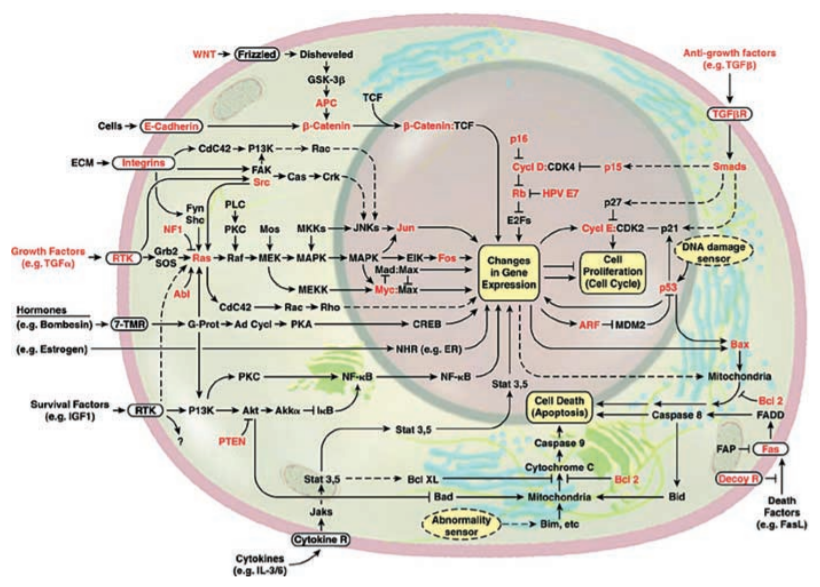
\includegraphics[width=0.6\textwidth]{figures/3-4.png}
        \end{figure}
    \end{frame}
    \section*{致谢}

    \begin{frame}
        \frametitle{致谢}
        \begin{columns}
            \begin{column}{.5\linewidth}
                我们的团队(排名不分先后):

                王泽州\quad 金皓宇\quad 陈齐治
        
                陈思元\quad 李鸿泽\quad 赵晨琪
                
                邓朝萌\quad 谭开云\quad 施朱鸣
            
                \bigskip

                感谢老师们和助教们的帮助!

                祝大家期中顺利,谢谢聆听!
            \end{column}
            \begin{column}{.5\linewidth}
                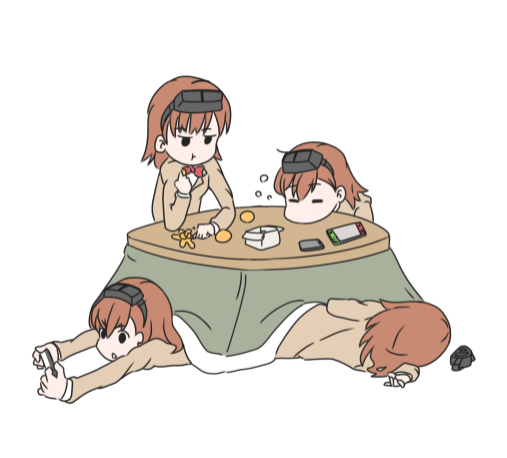
\includegraphics[width=.4\paperwidth]{figures/misaka558.png}
            \end{column}
        \end{columns}
        *\footnote{组长邮箱:shizhuming@pku.edu.cn \\ LaTeX代码开源在https://github.com/ShiZhuming/pku-cybernetics}
    \end{frame}
    
\end{document}